\section{Kolväten}
\subsection{Alkaner}
Alkaner är konväten som innehåller enbart enkla kovalenta bindningar mellan atomerna. De första 10 heter och ser ut som följande:
\begin{center}
    \tcbox[title={De 10 första - namn}]{\begin{tabular}{r c l}
            1. & Metan & \ce{CH4} \\
            2. & Etan & \ce{C2H6} \\
            3. & Propan & \ce{C3H8} \\
            4. & Butan & \ce{C4H10} \\
            5. & Pentan & \ce{C5H12} \\
            6. & Hexan & \ce{C6H14} \\
            7. & Heptan & \ce{C7H16} \\
            8. & Oktan & \ce{C8H18} \\
            9. & Nonan & \ce{C9H20} \\
            10. & Dekan & \ce{C10H22}
    \end{tabular}}
    \tcbox[title={De 10 första - struktur}]{\begin{tabular}{c >{\hspace{20pt}}c >{\hspace{20pt}}c}
        \chemfig{H-C([-2]-H)([2]-H)-H} & \chemfig{H-C([-2]-H)([2]-H)-C([-2]-H)([2]-H)-H} & \chemfig{H-C([-2]-H)([2]-H)-C([-2]-H)([2]-H)-C([-2]-H)([2]-H)-H} \\ \vspace{5pt} \\
        Metan & Etan & Propan
    \end{tabular}}
\end{center}
Dessa är mycket bra att komma ihåg. de första tre alkanerna med strukturformler syns även nedan.

\subsection{Arener}
En aren, alternativt ett aromatisk ämne, är ett cykliskt kolväte som binder med varannan binding dubbel. I mitten av denna ring kommer då elektronerna alltid att enbart kunna anta två olika konfigurationer. Detta leder till att de \emph{delokaliseras} och bildar ett ''medelvärde'' av deras positioner sen innan. De kommer alltså att finnas typ som ett samlat moln för alla kolatomer, likt en metallbindning. Det ser ut som följande för en hexanbas:
\begin{center}
    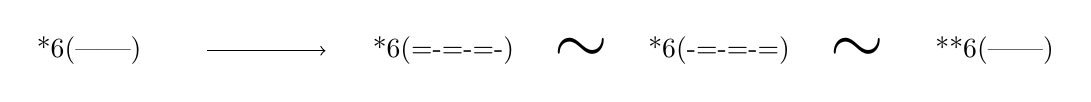
\begin{tikzpicture}
        \node at (-2.25,0) {\chemfig{*6(------)}};
        \draw[->] (0,00) ++(-1.5/2,0) -- ++(1.5,0);
        \draw (2.25,0) node {\chemfig{*6(=-=-=-)}} ++(2-0.25,0) node {\Huge{$\sim$}} ++(2-0.25,0) node {\chemfig{*6(-=-=-=)}} ++(2-0.25,0) node {\Huge{$\sim$}} ++(2-0.25,0) node {\chemfig{**6(------)}};
    \end{tikzpicture}
\end{center}

I detta fall innebär $\sim$ att något är samma molekyl som något annat. Denna aren för hexan kallas \emph{bensen}. Ringen i mitten ska illustrera detta medelvärde av elektroner och visar helt enkelt att det är ett aromatiskt ämne. Ett annat intressant aromatiskt ämne är \emph{grafen} vilket är en stor platta av sammanvävna kol-hexagoner med aromatiska bindningar som sedan har en kant av väte. Detta ser ut såhär:
\begin{center}
    \scalebox{0.8}{\chemfig[angle increment=30]{**6(([-3]**6(--([-5,0.5]-H)-([-3,0.5]-H)---))-(**6(--([-3,0.5]-H)-([-1,0.5]-H)---))-(**6(--([-1,0.5]-H)-([1,0.5]-H)---))-(**6(--([1,0.5]-H)-([3,0.5]-H)---))-(**6(--([3,0.5]-H)-([5,0.5]-H)---))-(**6(--([5,0.5]-H)-([7,0.5]-H)---))-)}}
\end{center}
I verkligheten expanderar detta mycket större, men i brist på plats är detta en lite del av en hypotetisk grafenskiva. Väte kommer enbart uppstå längs med kanterna på skivan.